
%  CONFIGURE NEW SINGLE-PAGE FORMAT 

\onecolumn % go back to one column
\fancyhead{} % make sure we get no headers
\renewcommand{\floatpagefraction}{0.1}
\lfoot[\bSupInf]{\dAuthor}
\rfoot[\dAuthor]{\cSupInf}
\newpage

\captionsetup*{format=largeformat} % make figure legend slightly larger than in the paper
\setcounter{figure}{0} % reset figure counter for Sup. Figures
\setcounter{equation}{0} % reset equation counter for Sup. Equations
\setcounter{table}{0} % reset equation counter for Sup. Equations
\setcounter{page}{1} % reset page count
\makeatletter
\renewcommand{\thefigure}{S\@arabic\c@figure} % make Figure legend start with Fig. S.
\makeatother
\makeatletter
\renewcommand{\thetable}{S\@arabic\c@table} % make Figure legend start with Fig. S.
\makeatother
\makeatletter
\renewcommand{\theequation}{S\@arabic\c@equation} % make Figure legend start with Fig. S.
\makeatother


% ------------------------------------------------------------------------------------------------------------------------------------


%\tableofcontents

\newpage
\section{Drift correction}
FluoCells slide \#2 (Thermo Fisher Scientific) were imaged on a Ti2 microscope (Nikon) (Fig. \ref{fig:DriftCorrection}) using a 100x TIRF objective (CFI Apochromat TIRF 100XC Oil, Nikon) onto a Prime 95B camera (Photometrics) in the GFP channel (tubulin), using an LED illumination source. 100 frames were acquired at 40 Hz and an artificially large drift was applied digitally.


\section{Channel alignment}

Multicolor beads (TetraSpeck™ Microspheres, 0.1 µm, fluorescent in blue/green/orange/dark red, Thermo Fisher Scientific) were prepared on a \#1.5 cover slip and embedded in water before being sealed with nail polish. The beads were then imaged on a Ti2 microscope (Nikon) (Fig. \ref{fig:ChannelAlignment}) using a 100x TIRF objective (CFI Apochromat TIRF 100XC Oil, Nikon) onto a Prime 95B camera (Photometrics), in both GFP and mCherry channels, using an LED illumination source. 

\section{SRRF}

\subsection{Cell lines}

Cos7 cells were cultured in phenol red-free Dulbecco’s modified Eagle’s medium (DMEM; Thermo Fisher Scientific) supplemented with 10\% (v/v) fetal bovine serum (FBS; Gibco), 1\% (v/v) penicillin/streptomycin (Thermo Fisher Scientific) and 2 mM L-alanyl-L-glutamine (GlutaMAX™, Thermo Fisher Scientific) at 37 \degree C in a 5\% CO\textsubscript{2} incubator.

\subsection{Sample preparation}

For live-cell imaging, Cos7 cells were seeded on 25mm-diameter \#1.5 coverslips (Marienfeld) at a density of 0.3 – 0.9×10\textsuperscript{5} cells/cm\textsuperscript{2}. One day after splitting, cells were transfected with a plasmid encoding the calponin homology domain of utrophin fused to GFP (GFP-UtrCH) \cite{burkel2007versatile} using Lipofectamin 2000 (Thermo Fisher Scientific) according to the manufacturer’s recommendations. Cells were imaged 1–4 days post transfection in culture medium.

\subsection{Imaging}

LED-illumination widefield imaging of GFP-UtrCH in live Cos7 cells (Fig. \ref{fig:SRRF}) was performed in at 37 °C and 5\% CO\textsubscript{2} on a N-STORM microscope (Nikon). A 100x TIRF objective (Apochromat 100x/1.49 Oil, Nikon) with additional 1.5x magnification was used to collect fluorescence onto an EMCCD camera (iXon Ultra 897, Andor), yielding a pixel size of 107 nm. Frames were acquired for 30 min with 30 ms exposure and 490 nm LED illumination at 5\% of maximum output. 

\subsection{SRRF reconstruction}

The dataset was reconstructed using NanoJ-SRRF with the following parameters: magnification: 5, radius: 0.5, number of axes: 6,  number of frames per SRRF reconstruction: 100, temporal analysis: Temporal Radiality Average (TRA). 


\section{SQUIRREL}

\subsection{Cell lines}
Cos7 cells were cultured as described in Supplementary Note 3.

\subsection{Sample preparation}

Cos7 cells were fixed with glutaraldehyde and labelled with two monoclonal mouse anti-alpha tubulin antibodies (DM1A and B-5-1-2, both from Sigma) and a goat anti-mouse Alexa Fluor 647-conjugated secondary antibody (A21235, Thermo Fisher Scientific). Samples were mounted in Smart Buffer (Abbelight) for imaging.

\subsection{STORM acquisition and reconstruction}

Imaging was performed on an N-STORM (Nikon) microscope using a 100x TIRF objective (Apochromat 100x/1.49 Oil, Nikon). Prior to STORM imaging, a reference widefield image was acquired using low intensity 642 nm laser excitation. For subsequent STORM imaging, 60,000 frames were acquired with high intensity 642 nm laser excitation at 15 ms exposure with pixel size of 160 nm and 0.1248 photons per analog-to-digital unit. Localizations were detected using the N-STORM software (Nikon), and exported as a text file to be rendered using ThunderSTORM \cite{ovesny2014thunderstorm}.

\subsection{SQUIRREL analysis}

The initially acquired widefield image was used as the reference and the ThunderSTORM reconstruction as the super-resolution image. All parameters in the plugin were left at their default values. For local resolution measurements, two independent super-resolution images were created using ThunderSTORM; one comprising of the localisations from odd-numbered frames, and the other of even-numbered frames. These images were concatenated to form a two slice image stack and the ‘Calculate FRC-map’ method of NanoJ-SQUIRREL was run with 10 blocks per axis.

\section{VirusMapper}

\subsection{Vaccinia virus sample preparation}
 
The L4-mCherry F17-EGFP virus was based on the WR strain and was described previously as WR EGFP-F17 VP8-mCherry \cite{schmidt2013vaccinia}. A4-EGFP was described previously as A5-EGFP \cite{schmidt2011vaccinia}. Virions were produced in BSC-40 cells, purified from cytoplasmic lysates and banded on a sucrose gradient. High performance coverslips (18x18 mm, \#1.5H Zeiss) were washed with water, ethanol and acetone sequentially three times, then sonicated for 20 min in 1 M potassium hydroxide. The purified virus was diluted in 1 \textmu{}L of 1 mM Tris buffer (pH 9) and placed onto the coverslips. After 30 min, virus solution was removed and the virus was fixed with 4\% formaldehyde in PBS for 20 min. Samples were washed 3 times with PBS and blocked for 30 min with 5\% BSA in PBS. A17 was stained with rabbit polyclonal anti-A17 antibody, which was a kind gift from Jacomine Krijnse-Locker (Institut Pasteur, Paris, France) and Alexa Fluor 647-conjugated secondary antibody (A21245, Thermo Fisher Scientific). For STORM imaging, A4-EGFP virus was bound to coverslips as described above. Samples were permeabilised with 0.2\% Triton-X 100 for 10 min, blocked 30 min with 5\% BSA in PBS and labelled with anti-L1 antibody 7D11, which was purified from a mouse hybridoma cell line kindly provided by Bernard Moss (NIH, Bethesda, MD) with permission of Alan Schmaljohn (University of Maryland, Baltimore, MD), and Alexa Fluor 647-conjugated secondary antibody (A21235, Thermo Fisher Scientific). 

\subsection{\textit{Sulfolobus acidocaldarius} sample preparation}

\textit{Sulfolobus acidocaldarius} strain DSM639 was grown in Brock’s medium (pH 3.2), supplemented with 0.1\% NZ-amine and 0.2\% sucrose at 75 ºC. Cells were fixed at OD600: 0.310 (i.e. within the limit of exponential growth) in 70\% EtOH, rehydrated in PBST (0.2\% v/v Tween) and stained overnight with polyclonal rabbit antibody for CdvB \cite{lindaas2008unique}. Secondary staining was done with Alexa Fluor 647-conjugated Concanavalin A-antibody (C21421, Thermo Fischer Scientific) for labelling the S-layer and Alexa Fluor 546-conjugated secondary goat anti-rabbit antibody (A11035, Thermo Fischer Scientific) for visualising CdvB. The cells were spun down onto 2\% polyethylenimine-coated coverslips before imaging.
 
\subsection{SIM imaging}

SR-SIM imaging of vaccinia virus was performed using a 63x objective (Plan-Apochromat 63x/1.4 oil DIC M27, Zeiss) and \emph{Sulfolobus} imaging was performed using a 100x TIRF objective (alpha Plan-Apochromat 100x/1.46 Oil DIC M27, Zeiss), both on an Elyra PS.1 microscope (Zeiss). Images were acquired using 5 phase shifts and 3 grid rotations, with the 647 nm (32 μm grating period) and 561nm (32 μm grating period) and the 488 nm (32 μm grating period) lasers, and filter set 3 (1850–553, Zeiss). 2D- (vaccinia) and 3D-images (\textit{Sulfolobus}) were acquired on an sCMOS camera and processed using ZEN Black software (Zeiss). Channels were aligned with the NanoJ-Core Channel Alignment Tool.

\subsection{SIM/STORM imaging}

Correlative SIM/STORM imaging of vaccinia virus (Fig. \ref{fig:VirusMapper}a, ref{fig:supVM|) was performed on a Zeiss Elyra PS.1 inverted microscope with a 100x TIRF objective (alpha Plan-Apochromat 100× /1.46 NA oil DIC M27, Zeiss) objective with a 1.6x tube lens and an iXon 897 EMCCD camera (Andor). SIM imaging was performed as described above. STORM images were acquired at 25-30 ms exposure with 642 nm excitation at 100\% laser power and a 655 nm LP filter. Activation was dynamically controlled with a 405 nm laser at 0-2\% laser power. Images were processed using ThunderSTORM \cite{ovesny2014thunderstorm}. Localisations were fitted with a maximum-likelihood estimator, lateral drift corrected by cross-correlation and localisations <20 nm apart within 2 frames merged.
 
\subsection{VirusMapper processing}

Individual viral particles or archaea cells were extracted from the SIM or SIM/STORM images. Template images were generated with VirusMapper as described previously \cite{gray2016virusmapper}. 2- or 3-colour models of vaccinia virus proteins and 2-colour models of \emph{Sulfolobus} S-layer and division ring in different orientations were then created by registration of the entire set of particles according to cross-correlation with the templates and calculation of a weighted average of a subset of particles. 

\section{NanoJ-Fluidics}

\subsection{Sample preparation}

Sample were prepared as described previously \cite{almada2018automating}. Briefly, Cos7 cells were grown, seeded on glass coverslips and then fixed as described in Supplementary Note 4 and were labelled with primary antibodies overnight: mouse monoclonal anti-TOM20 (612278, BD Biosciences), rabbit polyclonal anti-clathrin heavy chain (ab21679, Abcam) and chicken poly-clonal anti-vimentin (919101, BioLegend). Cells were then incubated with Exchange-PAINT secondary antibodies coupled to DNA sequences \cite{almada2018automating}: goat anti-mouse I1, goat anti-chicken I2 and goat anti-rabbit I3. After rinses, the cells were incubated with 12.5 μM Atto488-conjugated phalloidin (Merck) for 90 min at room temperature and imaged within 3-4 days. 

\subsection{NanoJ-Fluidics workflow and SMLM acquisition}

Imaging of Cos7 cells (Fig. \ref{fig:PAINT}) was performed as described in \cite{almada2018automating}. The NanoJ-Fluidics pump array was installed on an N-STORM microscope (Nikon) using a 100x TIRF objective (CFI Apochromat 100x/1.49 Oil, Nikon). First, a STORM imaging of phalloidin-Atto488 was performed using 30,000 frames at 30 ms exposure. After injection of the I1-Atto655 (0.25 nM) and I2-CY3B (2 nM) imager strands, 60,000 frames were acquired in an alternating way (30,000 frames of each channel) to image TOM20 and vimentin, respectively. After rinses, I3-Cy3B (1 nM) was injected, and 30,000 frames were acquired to image clathrin.

\subsection{SMLM reconstruction}

Localisations were detected using the N-STORM software (Nikon), and exported as a text file before being filting (number of photons between 700 and 50,000; number of detections (after linking across frames) < 50 frames) and rendered using ThunderSTORM.

\newpage

\begin{figure}
    \centering
    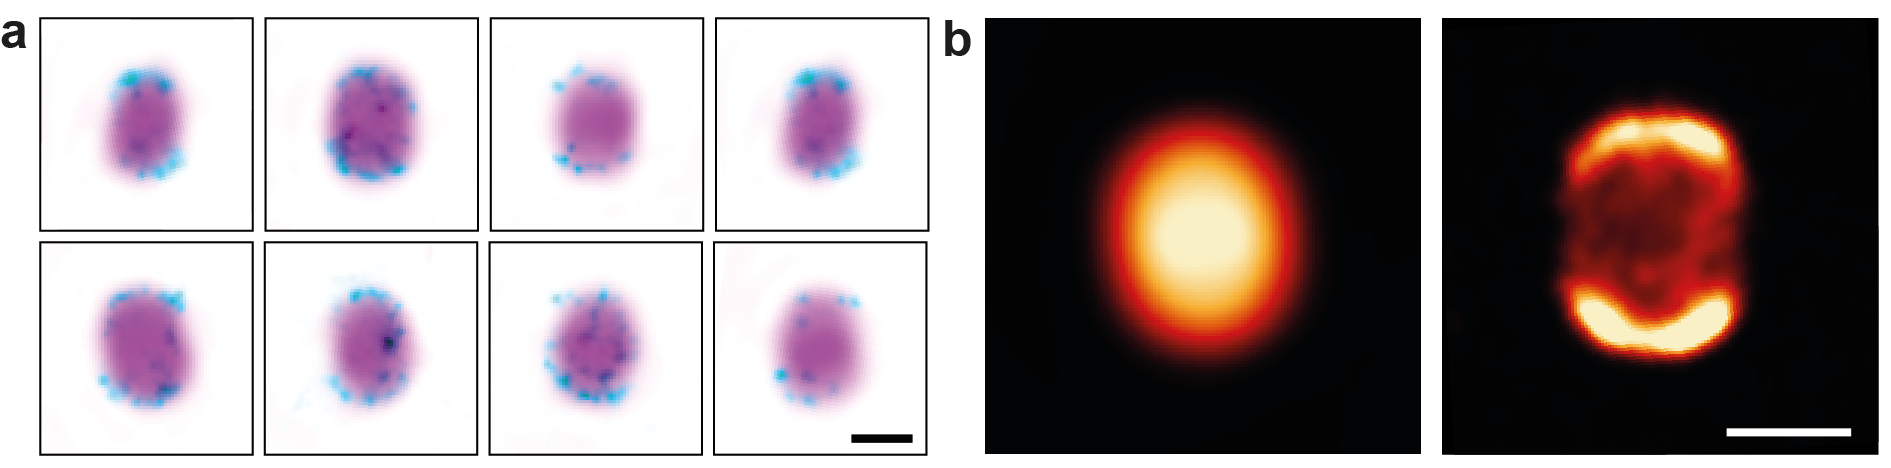
\includegraphics{Figures/dSTORM_Sup_L1.png}
    \caption{\textbf{NanoJ-VirusMapper analysis of SIM/SMLM data}. \textbf{a)} Example SIM/STORM images of A4-EGFP vaccinia virions labelled for the entry protein L1. SIM images were taken of the A4-EGFP core (magenta), followed by STORM images of the L1 membrane protein (cyan). The images were aligned and overlayed. \textbf{b)} VirusMapper SPA models of A4 and L1 using the SIM/STORM data. Particles were aligned in parallel and averaged to produce the model. Scale bars 200 nm.}
    \label{fig:supVM}
\end{figure}

\newpage
\section*{Bibliography}
\bibliographystyle{zHenriquesLab-StyleBib}
\bibliography{06_Bibliography_Clean}

